\documentclass[aspectratio=169]{beamer}
\mode<presentation>{
\usetheme{default}
}

\usepackage{graphicx} 
\usepackage{booktabs} 
\usepackage{graphicx,color}
\usepackage{minted} %extrai python com sitaxe destacada

\title[Short title]{Neural Nets with Keras} 
\subtitle{Intel-Unesp/NCC - Machine Learning and High Performance Computing Team}
\author{Machine Learning Team}

\begin{document}
\begin{frame}
\titlepage 
\end{frame}

\begin{frame}
\frametitle{Overview} 
\begin{itemize}
\item Introduction to Keras: The Python Deep Learning Library
\item Sequential Model
\item Model Class API
\item Sequential Model: Recognizing Handwritten Digits (Single and MLP Nets)
\item Optimizers in Keras
\item How to Avoid Overfitting!
\item Introduction to Convolutional Nets
\end{itemize}
\end{frame}

%-S1
\begin{frame}
\frametitle{Keras:The Python Deep Learning library}
Keras is a high-level neural networks API, written in Python and capable of running on top of either TensorFlow, CNTK or Theano.
\\[0.5cm]
Keras is compatible with: Python 2.7-3.6.
\end{frame}
%-S1

%-S2
\begin{frame}
\frametitle{Sequential Model}
The initial building block of Keras is a model, and the simplest model is called \textcolor{red}{sequential}. 
\\[0.6cm]
A sequential Keras model is a linear pipeline \textcolor{blue}{(a stack)} of \textbf{neural networks layers}.
\\[0.6cm]
An example of a Neural Net in Keras:
\\[0.3cm]
The code below defines a single (dense) layer with \textcolor{red}{12} artificial neurons, and \textcolor{blue}{8} input variables (\textbf{features}):
\\[0.3cm]
%-------------Input python-------
\inputminted{python}{./aux_files/one.py}
%--------------------------------
\end{frame}
%-S2

%-S3
\begin{frame}[fragile]
\frametitle{Sequential Model}
\textbf{Kernel Initializer} 
\\[0.6cm]
Each neuron can be initialized with specific weights.
\\[0.3cm]
Keras provides a few choices, the most common of which are:
\begin{itemize}
\item \begin{verbatim}'random_uniform': Weights are initialized to 
uniformly random small values in (-0.05, 0.05)\end{verbatim}  
\item \begin{verbatim}'random_normal': Weights are initialized according 
to a Gaussian, with a zero mean and small standard 
deviation of 0.05.\end{verbatim}
\item \begin{verbatim}zero: All weights are initialized to zero.\end{verbatim}
\end{itemize}
\textcolor{red}{Find out more in: https://keras.io/initializations/.} 
\end{frame}
%-S3

%-S4
\begin{frame}
\frametitle{Sequential Model}
\textbf{Compilation}:
Before training a model it is necessary to configure the learning process. It is done by \textcolor{red}{compile} method. 
\\[0.5cm]
This method receives three arguments:
\\[0.3cm]
\begin{enumerate}
\item An Optimizer such as \textcolor{blue}{rmsprop or adam};
\\[0.3cm]
\item  Objective Function - \textcolor{red}{"loss function"}. This is the objective that the model will try to minimize;
\\[0.3cm]
\item A list of metrics: \textcolor{red}{metrics=['accuracy']}.
\end{enumerate}
\end{frame}
%-S4

%-S5
\begin{frame}
\frametitle{Sequential Model}
\textbf{Compilation}
\\[0.5cm]
\begin{itemize}
\item \textit{For a multi-class classification problem}
\inputminted{python}{./aux_files/two.py}
\end{itemize}
\end{frame}
%-S5

%-S6
\begin{frame}
\frametitle{Sequential Model}
\textbf{Compilation}
\\[0.5cm]
\begin{itemize}
\item \textit{For a binary classification problem}
\inputminted{python}{./aux_files/three.py}
\end{itemize}
\end{frame}
%-S6

%-S7
\begin{frame}
\frametitle{Sequential Model}
\textbf{Compilation}
\\[0.5cm]
\begin{itemize}
\item \textit{For regression  problem}
\inputminted{python}{./aux_files/four.py}
\end{itemize}
\end{frame}
%-S7

%-S8
\begin{frame}
\frametitle{Sequential Model}
\textbf{Training}
\\[0.1cm]
\begin{itemize}
\item \textit{Keras runs over Numpy!}
\item \textit{For training a model use the \textcolor{red}{fit} function}.
\end{itemize}
\textbf{\textit{For binary classification}:}
\inputminted{python}{./aux_files/six.py}
\end{frame}
%-S8

%-S9
\begin{frame}
\frametitle{Sequential Model}
\textbf{Training}
\\[0.5cm]
\textbf{\textit{For categorical classification}:}
\inputminted{python}{./aux_files/seven.py}
\end{frame}
%-S9

%-S10
\begin{frame}
\frametitle{Sequential Model}
\textbf{Example from https://keras.io/getting-started/sequential-model-guide/}
\\[0.3cm]
Multilayer Perceptron (MLP) for multi-class \textit{\textcolor{red}{softmax}} classification:
\\[0.3cm]
\textit{Inserting Headers}
\inputminted{python}{./aux_files/eight.py}
\end{frame}
%-S10

%-S11
\begin{frame}
\frametitle{Sequential Model}
\textit{Creating Dummy Data}
\inputminted{python}{./aux_files/nine.py}
\end{frame}
%-S11

%-S12
\begin{frame}
\frametitle{Sequential Model}
\textit{Creating a MLP Neural Net}
\inputminted{python}{./aux_files/ten.py}
\end{frame}
%-S12

%-S13
\begin{frame}
\frametitle{Sequential Model}
\textit{Compiling the Neural Net Model}
\inputminted{python}{./aux_files/eleven.py}
\end{frame}
%-S13

%-S14
\begin{frame}
\frametitle{Sequential Model}
\textit{Training/Evaluating the Neural Model}
\inputminted{python}{./aux_files/twelve.py}
\end{frame}
%-S14

%-S15
\begin{frame}
\frametitle{Model Class API}
In the functional API, you can create a Model via:
\\[0.2cm]
\inputminted{python}{./aux_files/thirteen.py}
Note that his model include all layers required in the computation of \textcolor{red}{a} given \textcolor{blue}{b}
\end{frame}
%-S15

%-S16
\begin{frame}
\frametitle{Model Class API}
In the case of multi-input multi-output models, we can use:
\\[0.2cm]
\inputminted{python}{./aux_files/fourteen.py}
\end{frame}
%-S16

%-S17
\begin{frame}
\frametitle{Recognizing Handwritten Digits!}
In this section we build a network that can recognize Handwritten Digits.
\\[0.3cm]
For this, it will be used the MNIST Database (http://yann.lecun.com/exdb/mnist/), a set made up of 60.000 examples and a test set of 10.000 examples.
\\[0.3cm]
This training examples are annotated by humans with the correct answer. If the handwritten digit is the number three, then three is simply the label associated with that example.
\begin{figure}
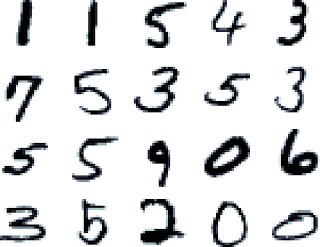
\includegraphics[width=2cm,height=2cm]{./aux_files/one.jpg}
\caption{MNIST Digits}
\label{fig:MNIST Digits}
\end{figure}
\end{frame}
%-S17

%-S18
\begin{frame}
\frametitle{Recognizing Handwritten Digits!}
Step 1 - Spliting the Data Set
\inputminted{python}{./aux_files/fifteen.py}
\emph{X\_train has 60000 samples of 28x28, reshaped in 60000x784 inputs}
\end{frame}
%-S18

%-S19
\begin{frame}
\frametitle{Recognizing Handwritten Digits!}
Step 2 - Modeling the Net
\inputminted{python}{./aux_files/sixteen.py}
\emph{The input layer has a neuron for each picel in the image (784 neurons) and the final layer has a single neuron with softmax activation - a generalization of sigmoid functions}
\end{frame}
%-S19

%-S20
\begin{frame}
\frametitle{Recognizing Handwritten Digits!}
Step 2 - Compiling the Net
\inputminted{python}{./aux_files/seventeen.py}
\emph{The compiled model now can be executed by Keras over Theano or TensorFlow}
\end{frame}
%-S20

%-S21
\begin{frame}
\frametitle{Recognizing Handwritten Digits!}
Step 2 - Training the Net
\inputminted{python}{./aux_files/eighteen.py}
\textbf{Remember!:}
\\[0.5cm]
\emph{\textcolor{red}{epochs}:the number of times the model is exposed to the training set; \textcolor{blue}{batch\_size}:number of training instances observed before the optimizer performs a weight update.}
\end{frame}
%-S21

%-S21
\begin{frame}
\frametitle{Recognizing Handwritten Digits!}
Step 2 - Evaluating the Model 
\inputminted{python}{./aux_files/nineteen.py}
\emph{Now we can evaluate the neural model on the test set that contains new \textit{\textbf{\textcolor{blue}{unseen}}} examples. }
\\[0.2cm]
\textcolor{red}{Note that the training set and the test set are rigorously separated. Learning is a process intended to generalize unseen observationsand not to memorize what is already know!}
\end{frame}
%-S21

%-S21
\begin{frame}
\frametitle{Recognizing Handwritten Digits!}
Step 2 - \textcolor{red}{Run the Source Code}
\\[0.5cm]
\emph{Code: NeuralNetpy - https://github.com/julioaamaral/ml/blob/master/NeuralNet.py}
\\[0.3cm]
\textbf{Results got with 50 epochs: loss: 0.3289; accuracy:0.9087}
\\[0.3cm]
\textcolor{red}{Check it out and try to improve them! - Test this code with others parameters!}
\end{frame}
%-S21

%-S21
\begin{frame}
\frametitle{Hidden Layers}
Step 2 - \textcolor{red}{MultiLayer Perceptron in Keras}
\\[0.5cm]
\inputminted{python}{./aux_files/twenty.py}
\end{frame}
%-S21

%-S21
\begin{frame}
\frametitle{Recognizing Hanwritten Digits!}
Step 2 - \textcolor{red}{Run the Source Code}
\\[0.5cm]
\emph{Code: MLP.py - https://github.com/julioaamaral/ml/blob/master/MLP.py}
\\[0.3cm]
\textbf{Results got with 50 epochs: loss: ? accuracy:?}
\\[0.3cm]
\textcolor{red}{Check it out and try to improve them! - Test this code with others parameters!}
\end{frame}
%-S21

%-S21
\begin{frame}
\frametitle{Hidden Layers}
Step 2 - \textcolor{red}{MultiLayer Perceptron (with Dropout) in Keras}
\\[0.5cm]
\inputminted{python}{./aux_files/twentyone.py}
\end{frame}
%-S21

%-S21
\begin{frame}
\frametitle{Recognizing Hanwritten Digits!}
Step 2 - \textcolor{red}{Run the Source Code}
\\[0.5cm]
\emph{Code: MLP\_Dropout.py - https://github.com/julioaamaral/ml/blob/master/MLP\_Dropout.py}
\\[0.3cm]
\textbf{Results got with 50 epochs: loss: ? accuracy:?}
\\[0.3cm]
\textcolor{red}{Check it out and try to improve them! - Test this code with others parameters!}
\end{frame}
%-S21



%-S21
\begin{frame}
\frametitle{Testing different optimizers in Keras}
\inputminted{python}{./aux_files/twentytwo.py}
\end{frame}
%-S21

%-S21
\begin{frame}
\frametitle{Testing different optimizers in Keras}
\emph{Hands On!}
Run the code \textcolor{red}{\textbf{MLP\_Dropout.py}} using differents optimizers!
\\[0.3cm]
Code address: https://github.com/julioaamaral/ml/blob/master/MLP\_Dropout.py
\end{frame}
%-S21

%-S21
\begin{frame}
\frametitle{Regularization for Avoid Overfitting}
keras offers different types of regularization. Take a look! 
\\[0.3cm]
\begin{itemize}
\item \textcolor{red}{L1 - also know as \textbf{lasso}}
\item \textcolor{red}{L2 - also know as \textbf{ridge}}
\item \textcolor{red}{Elastic net regularization}
\\[0.3cm]
Note that the same ideia of regularization can be applied indepentently to the weights, to the model, and to the activation.
\inputminted{python}{./aux_files/twentythree.py} 
\end{itemize}
\end{frame}
%-S21

%-S21
\begin{frame}
\frametitle{Predicting Output}
\textbf{\emph{When a net is trained, it can be used for prediction. In Keras we use the following method:}}
\inputminted{python}{./aux_files/twentyfour.py}
\end{frame}
%-S21

%-S21
\begin{frame}
\frametitle{An Introduction to Convolutional Nets}
Convolutional neural networks (also called ConvNet) leverage spatial information and are therefore very well suited for classifying images.
\\[0.3cm]
These nets use an ad hoc architecture inspired by biological data taken from physiological experiments doneon the visual cortex. 
\\[0.3cm]
Note that our vision system is based on multiple cortex levels; each one applied on recognizing more and more structured information. From single pixels to sophisticated elements such as objects, faces, etc. 
\end{frame}
%-S21

%-S17
\begin{frame}
\frametitle{Deep Convolutional Neural Nets - DCNN}
A \textbf{\emph{\textcolor{red}{Deep Convolutional Neural Net}}} consist of many neural layers. Two different types \textcolor{blue}{convolutional} and \textcolor{blue}{pooling} as typically used alternated.
\begin{figure}
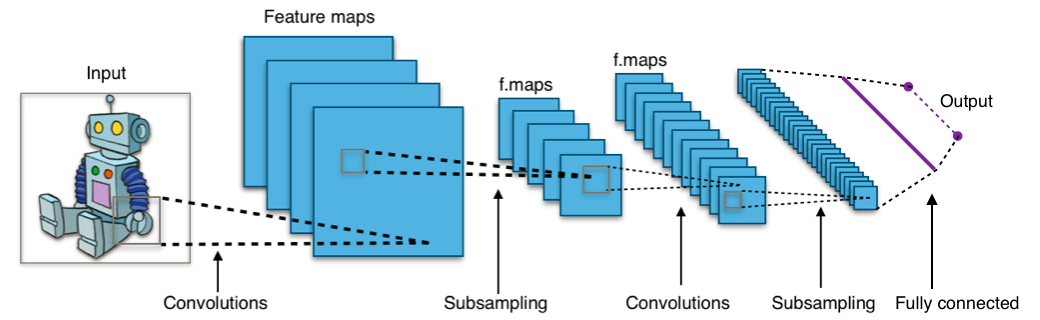
\includegraphics[width=15cm,height=4cm]{./aux_files/two.jpg}
\caption{ConvNet}
\label{fig:ConvNet Digits}
\end{figure}
\end{frame}
%-S17

%-S21
\begin{frame}
\frametitle{Modeling ConvNets}
\textbf{\emph{In Keras, to add a convolutional layer with dimensionality of the output 32 and kernel with 3x3, we use:}}
\inputminted{python}{./aux_files/twentyfive.py}
or 
\inputminted{python}{./aux_files/twentysix.py}
\end{frame}
%-S21

%-S21
\begin{frame}
\frametitle{Modeling ConvNets}
\textbf{Note that the input (image) in the last example has shape (256,256).}
\\[0.3cm]
\emph{With \textcolor{red}{TensorFlow} this input, consider three channels (RGB), is represented as (256,256,3) and with \textcolor{blue}{Theano}, (3,256,256).}
\end{frame}
%-S21

%-S21
\begin{frame}
\frametitle{Modeling ConvNets}
\textbf{\emph{Max-Pooling}}
\\[0.1cm]
One  common choice for \emph{Pooling} Layer is \textcolor{red}{max-pooling}, which simply outputs the maximum activation as observed in the region. In Keras, to define a max-pooling layer of size 2 x 2, we code:
\inputminted{python}{./aux_files/twentyseven.py}
\begin{figure}
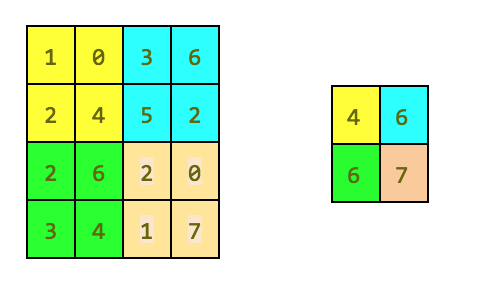
\includegraphics[width=5cm,height=2cm]{./aux_files/three.jpg}
\caption{MaxPooling Filter}
\label{fig:MaxPooling Filter- Shaped(2x2)}
\end{figure}
\end{frame}
%-S21

%-S21
\begin{frame}
\frametitle{An example of DCNN - LeNet}
Yann le Cun proposed  a family of ConvNets named LeNet trained for recognizing MNIST handwritten characters with robustness to simple geometric transformations and to distortion. 
\\[0.3cm]
The key intuition here is to have low-layers alternating convolution operations with max-pooling operations. 
\\[0.3cm]
The convolution operations are based on carefully chosen local receptive fields with shared weights for multiple feature maps. 
\\[0.3cm]
Higher levels are fully connected layers based on a traditional MLP with hidden layers and softmax as the output layer.
\textit{Take a look at: \textcolor{red}{Convolutional Networks for Images, Speech, and Time-Series, by Y. LeCun and Y. Bengio, brain theory neural networks, vol. 3361, 1995}}
\end{frame}
%-S21

%-S21
\begin{frame}
\frametitle{LeNet in Keras}
\textbf{To define LeNet code, we use a convolutional 2D module, which is:}
\inputminted{python}{./aux_files/twentyeight.py}
\textbf{In addition, we use a \textcolor{red}{MaxPooling2D} layer:}
\inputminted{python}{./aux_files/twentynine.py}
\end{frame}
%-S21

%-S21
\begin{frame}
\frametitle{Coding the LeNet - Layers}
\emph{Inserting  modules:}
\inputminted{python}{./aux_files/thirty.py}
\end{frame}
%-S21

%21
\begin{frame}
\frametitle{Coding the LeNet - Layers}
\emph{Defining the Net:}
\inputminted{python}{./aux_files/thirtyone.py}
\end{frame}
%-S21

%21
\begin{frame}
\frametitle{Coding the LeNet - Layers}
\emph{Defining the Net:}
\inputminted{python}{./aux_files/thirtytwo.py}
\end{frame}
%-S21

%21
\begin{frame}
\frametitle{Coding the LeNet - Layers}
\emph{Defining the Net:}
\inputminted{python}{./aux_files/thirtythree.py}
\end{frame}
%-S21

%21
\begin{frame}
\frametitle{Coding the LeNet - Layers}
\emph{Topology of the Net:}
\begin{figure}
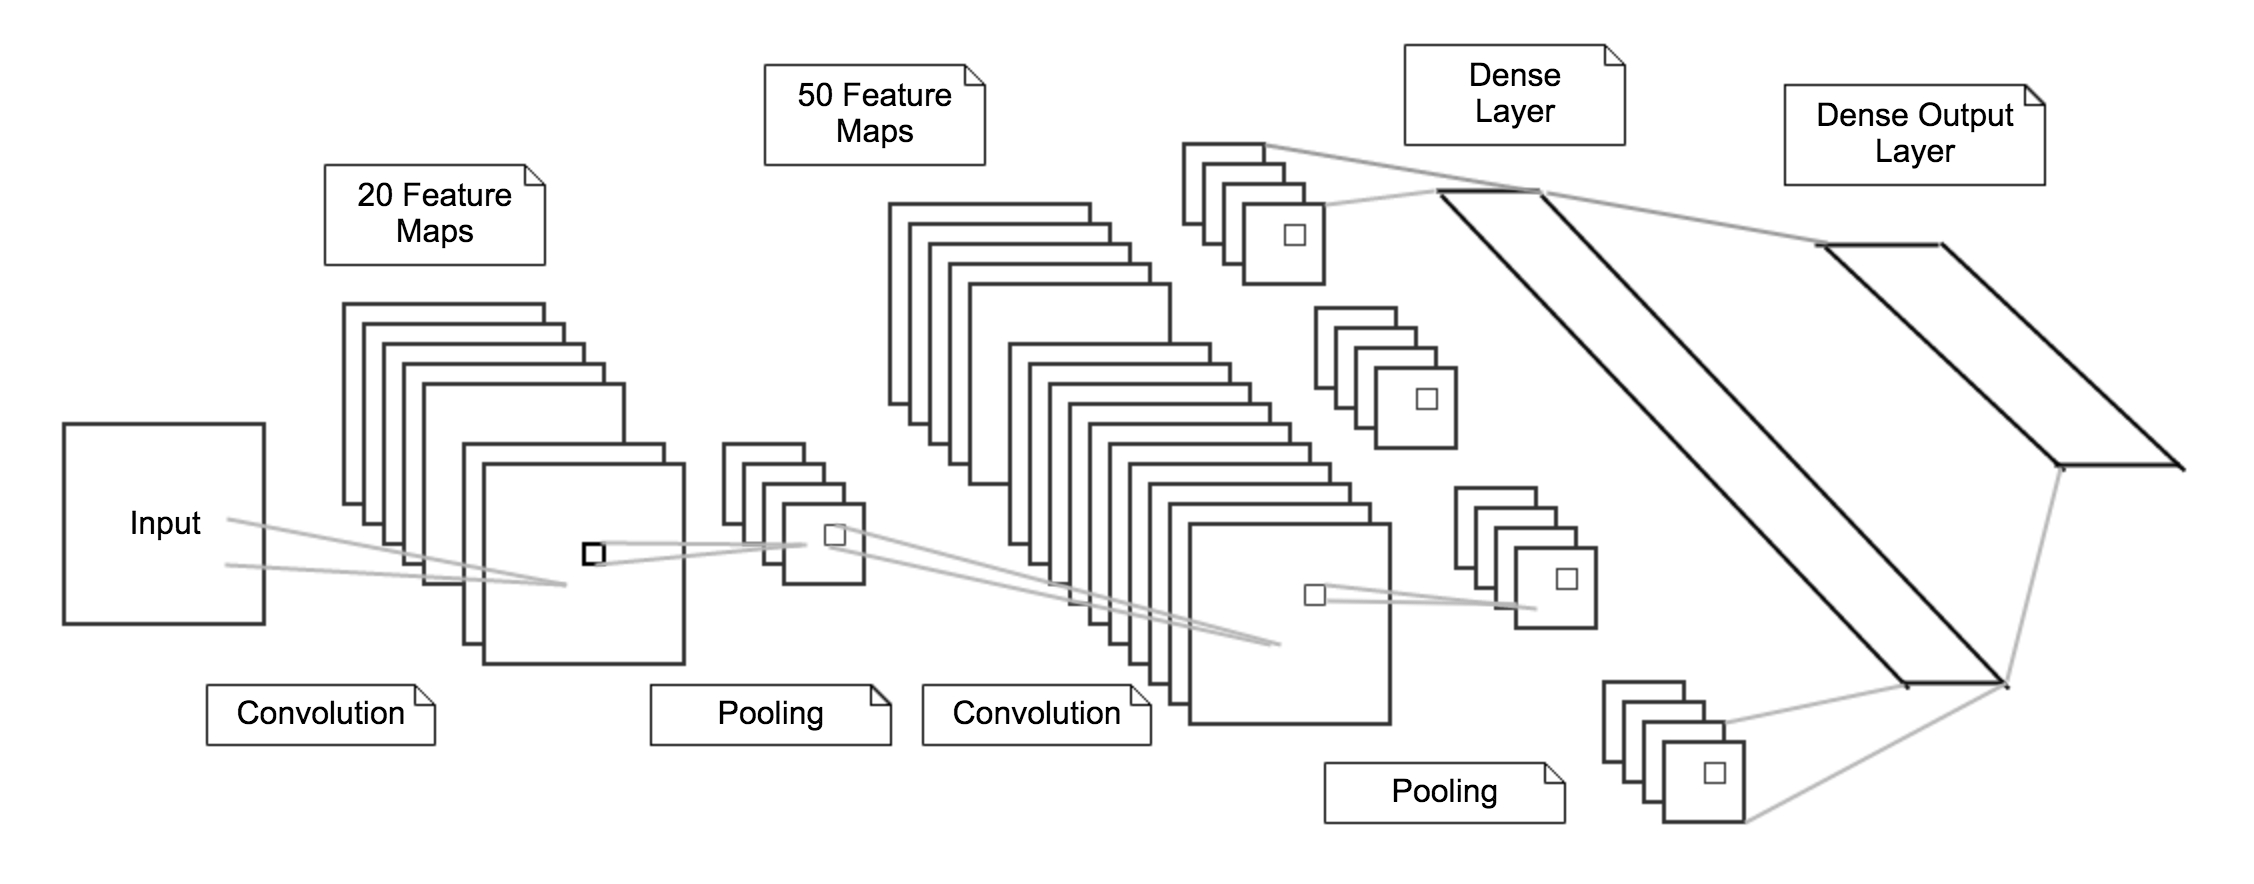
\includegraphics[width=12cm,height=6cm]{./aux_files/four.jpg}
\caption{LeNet}
\label{fig:LeNet Topology}
\end{figure}
\end{frame}
%-S21

%-S21
\begin{frame}
\frametitle{LeNet - HandsOn!}
\emph{Hands On!}
Run the code \textcolor{red}{\textbf{LeNet.py}}! 
\\[0.5cm]
\emph{Code: LeNet.py - https://github.com/julioaamaral/ml/blob/master/LeNet.py}
\\[0.3cm]
\textbf{Results got with 20 epochs: loss: ? accuracy:?}
\\[0.3cm]
\textcolor{red}{Check it out and try to improve them! - Test this code with others parameters!}
\end{frame}
%-S21

\begin{frame}
\frametitle{References}
\footnotesize{
\begin{thebibliography}{99} 
\bibitem[HAYKIN, 2012]{p1} HAYKIN, S. Neural Netwoks, NJ:Prentice Hall, 2009
\bibitem[Keras.io - Online Keras Documentation]{p2} Keras Documentation - https://keras.io/
\end{thebibliography}
}
\end{frame}
\end{document}
